\section{Introduction}\label{sec:intro}

Affective computing is an emerging interdisciplinary research field ranging from cognitive and social sciences to human-computer interaction (HCI) researchers with techniques like computer vision, machine learning, natural language understanding, etc.
With the long-term research on emotion theory from psychology and neuroscience~\cite{james1884emotion, turkle2005second}, emotion has been confirmed to be a significant effect \cite{james2013emotion} on human communication, decision making and perception.

On the perspective of human-computer interaction, Picard~\cite{picard1999affective} pointed out that affective computing (involved projects) can be used for \emph{reducing user frustration}, enabling comfortable communication of user emotion, developing infrastructure and applications to \emph{handle affective information}, as well as building tools that \emph{help formulate social-emotional skills}.

Recently, the ubiquitous computing~\cite{weiser1991computer} and wearable computing~\cite{starner1996human}, which are strictly related to affective computing, have achieved the pervasive attention of scientists. Ubiquitous computing and wearable computing are the necessary products of the combination of mobile computing technology and computer individualization.

Hence, it creates new research opportunities for affective computing that inferring user emotions with the combination of smart mobile wearable devices. We simply call it \emph{Mobile Affective Inference}. Such devices have been widely used over the world. The key feature of smart devices is the abundant sensors that enable unobtrusive monitoring of various affect-related signals. Exploring the possibility of using smart mobile devices for affective computing will benefit at least three perspectives by the potential of long-term unobtrusive monitoring user’s affective states: First, it influences the affect-related research literature by the wild, natural and unobtrusive study; Second, it establishes the spontaneous affect databases efficiently to evaluate new effective methods, models, systems more accurately; and third, it enhances the user-centered HCI design for the future ubiquitous computing environments.

In this paper, we present an introduction to the mobile affective computing techniques. Our next section discusses existing data sources from mobile devices, and Section~\ref{sec:methods} illustrate the recent advances for each different type of data and present the state-of-the-art model and method. Next Section~\ref{sec:applications}, based on the previous information (we reasonably assume we have finished user emotion inference stage), then gives two typical HCI applications in this field. At last, Section~\ref{sec:challenges} and~\ref{sec:conclusion} discuss the current challenges of mobile affective inference and our conclusion of this introduction.
Figure~\ref{fig:hierarchically} shows the hierarchically-structured taxonomy of this paper.

\begin{figure}[htb]
    \centering
    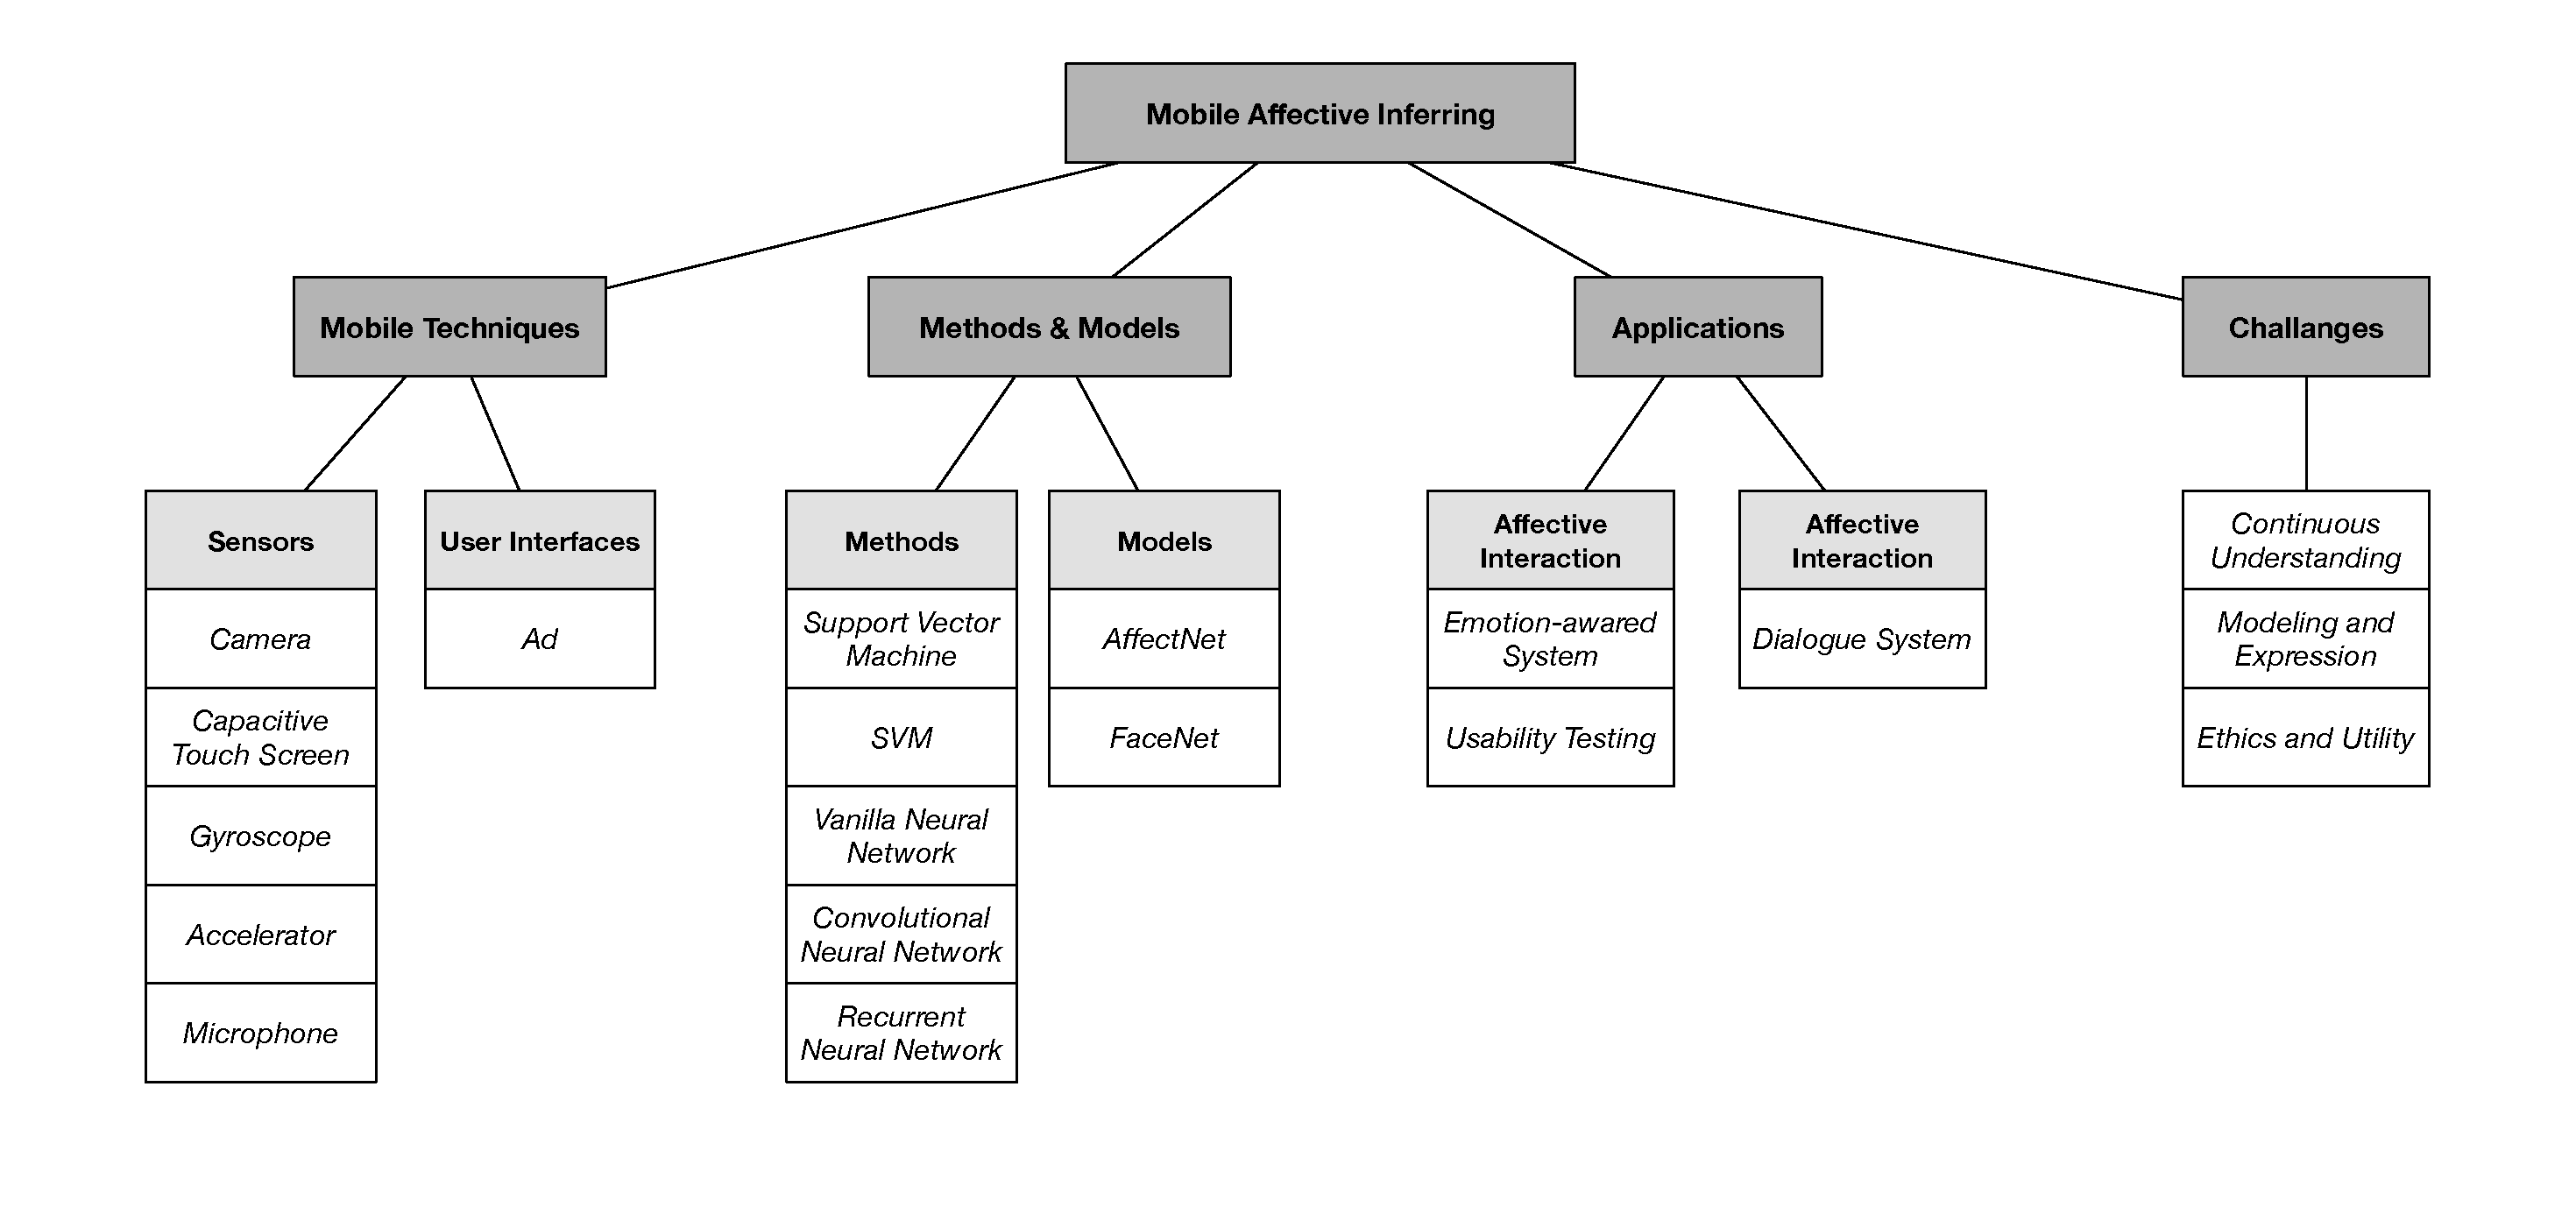
\includegraphics[width=0.5\textwidth]{hierarchical}
    \caption{Hierarchically-structured taxonomy of this paper.}
    \label{fig:hierarchically}
\end{figure}